% Sample file for 'CACM - Research Highlights'-type articles
% Created by: Gerry Murray, Elec. Pub. Info. Mgr., Pubs. Dept., ACM HQ, NY.
% (murray@hq.acm.org)
%
% This is "research-highlights-sample.tex" (sample file) V1.1 Sept. 2008
% This file should be compiled with V1.1 of "research4cacm.cls" Sept. 2008
%
% If you have already submitted an article to an ACM/SIGS Conference, and have had your
% article published in one of the 'Proceedings', then you have probably used
% the (ACM/SIGS) 'sig-alternate' class and .tex file.
% Any such 'conference-prepared' source .tex file is 'compatible' with the class file
% 'research4cacm' which you will use to prepare your article for inclusion in the magazine 'CACM'.
%
% Here are the steps to take in order to 'morph' your article from being
% a 'conference' article to one more suitable for inclusion in 'Communications of the ACM'.
%
% 1. Change \documentclass{sig-alternate}  to \documentclass{research4cacm}
%
% 2. Comment out the conference information e.g.  %\conferenceinfo{WOODSTOCK}{'97 El Paso, Texas USA}
%
% 3. Make sure the copyright data is correct e.g. \crdata{0001-0782/08/0200}
%
% 4. Make sure the YEAR is correct e.g. \CopyrightYear{2008} with the current default being �2008�.
%
% 5. Comment out the Classification scheme, general terms and keywords.
%
% 6. If you have mentioned authors in the 'Additional Authors' section you should
%    'move them back' into the byline (so that they appear with all the other authors).
%    ALL authors, in Research Highlights articles, get equal billing.
%
% 7. Suitably edit the file (i.e. body text) so as to make it more appropriate for a wider audience.
%
% If, early on in the editorial process, the 'correct' copyright data becomes available
% please change the copyright data to suit, otherwise leave the default '0001-0782/08/0X00'.
% (The editorial staff will change it later on in the production cycle.)
%
% ================= IF YOU HAVE QUESTIONS =======================
% Technical questions _only_ to
% Gerald Murray (murray@hq.acm.org)
% ===============================================================
% ---------------------------------------------------------------------------------------------------------------
%
\documentclass{research4cacm}
\begin{document}
%
% --- Author Metadata here ---
% Conference information is NOT appropriate for CACM so comment it out.
%\CopyrightYear{2008} % Allows default copyright year (2008) to be over-ridden - IF NEED BE.
%\crdata{0001-0782/08/0X00}  % Allows default copyright data (0001-0782/08/0X00) to be over-ridden - IF NEED BE.
% --- End of Author Metadata ---

\title{Sample `Research Highlights' article for publication\\ in {\ttlit CACM} in LaTeX Format
% \titlenote{(This is a simple titlenote.)For use with research4cacm.cls. Supported by ACM.}
%
% Show use of \thanks - which can appear here (normal/default) or down by the author
\thanks{The original version of this paper is entitled ``XXX" and was
published in (Title of publication, publication date, publisher.)}
}
\subtitle{[Extended Abstract]
%\titlenote{A full version of this paper is available in...}
}
%
% You need the command \numberofauthors to handle the 'placement
% and alignment' of the authors beneath the title.
%
% For aesthetic reasons, we recommend 'three authors at a time'
% i.e. three 'name/affiliation blocks' be placed beneath the title.
%
% NOTE: You are NOT restricted in how many 'rows' of
% "name/affiliations" may appear. We just ask that you restrict
% the number of 'columns' to three.
%
% Use the \alignauthor commands to handle the names
% and affiliations.
%
\numberofauthors{6} %  in this sample file, there are a *total*
% of SIX authors and all of them fit neatly on the first page.
% As said, all authors get 'equal billing' and you should fit all of them on the opening page
% in the 'byline'. The production/editorial-staff will 'separate' names from their affiliations, leaving
% author names beneath the title (in the byline), and moving the affilations/contact information to an area
% after the references at the back of the article.
%
\author{
% You can go ahead and credit any number of authors here,
% e.g. one 'row of three' or two rows (consisting of one row of three
% and a second row of one, two or three).
%
% The command \alignauthor (no curly braces needed) should
% precede each author name, affiliation/snail-mail address and
% e-mail address. Additionally, tag each line of
% affiliation/address with \affaddr, and tag the
% e-mail address with \email.
%
% 1st. author
\alignauthor
Ben Trovato\titlenote{A note from Dr.~Trovato.}\\
       \affaddr{Institute for Clarity in Documentation}\\
       \affaddr{1932 Wallamaloo Lane}\\
       \affaddr{Wallamaloo, New Zealand}\\
       \email{trovato@corporation.com}
% 2nd. author
\alignauthor
G.K.M. Tobin\titlenote{A note from G. Tobin.}\\
       \affaddr{Institute for Clarity in Documentation}\\
       \affaddr{P.O. Box 1212}\\
       \affaddr{Dublin, Ohio 43017-6221}\\
       \email{webmaster@marysville-ohio.com}
% 3rd. author
\alignauthor Lars Th{\o}rv{\"a}ld\titlenote{A note from Lars.}\\
       \affaddr{The Th{\o}rv{\"a}ld Group}\\
       \affaddr{1 Th{\o}rv{\"a}ld Circle}\\
       \affaddr{Hekla, Iceland}\\
       \email{larst@affiliation.org}
\and  % use '\and' if you need 'another row' of author names
% 4th. author
\alignauthor Lawrence P. Leipuner\\
       \affaddr{Brookhaven Laboratories}\\
       \affaddr{Brookhaven National Lab}\\
       \affaddr{P.O. Box 5000}\\
       \email{lleipuner@researchlabs.org}
% 5th. author
\alignauthor Sean Fogarty\\
       \affaddr{NASA Ames Research Center}\\
       \affaddr{Moffett Field}\\
       \affaddr{California 94035}\\
       \email{fogartys@amesres.org}
% 6th. author
\alignauthor Charles Palmer\\
       \affaddr{Palmer Research Laboratories}\\
       \affaddr{8600 Datapoint Drive}\\
       \affaddr{San Antonio, Texas 78229}\\
       \email{cpalmer@prl.com}
}

\maketitle
\begin{abstract}

This paper (and accompanying class file) provide a typical example of a \LaTeX\ document which
would be suitable for publication in the \textit{Research Highlights} section of \textit{CACM}.

The style closely mirrors the formatting guidelines for ACM Proceedings so \textit{morphing}
a \textit{Proceedings} article into one suitable for publication in \textit{CACM} should be minimal.
Just as for Proceedings, it is an {\em alternate} style which produces
a {\em tighter-looking} paper and was designed in response to
concerns expressed, by authors, over page-budgets.
It complements the document \textit{Author's Guide to
Preparing CACM Research Hightlights articles Using \LaTeX$2_\epsilon$\ and Bib\TeX}.
This source file has been written with the intention of being
compiled under \LaTeX$2_\epsilon$\ and BibTeX.

The developers have tried to include every imaginable sort
of ``bells and whistles", such as a subtitle, footnotes on
title, subtitle and authors, as well as in the text, and
every optional component (e.g. Acknowledgments, Additional
Authors, etc.), not to mention examples of
equations, theorems, tables and figures.

To make best use of this sample document, run it through \LaTeX\
and BibTeX, and compare this source code with the printed
output produced by the dvi file. A compiled PDF version
is available on the web page to help you with the
`look and feel'.
\end{abstract}

% The classification Scheme, General Terms and Keywords are not appropriate for CACM so comment them out.

\section{Introduction}
Articles cited to be published in the \textit{Research Highlights} section, of \textit{CACM},
will provide readers with a collection of outstanding research articles, selected from the
broad spectrum of computing-research conferences. Submissions for this section are
first nominated by Editorial Board Members or Approved Nominating Organizations, and are
then subject to final selection by the Editorial Board. Authors are then invited to
submit their article, \textit{after they have rewritten and expanded the scope of their articles}
as appropriate for the broad readership of \textit{Communications}. It is important
to note that publication in \textit{Communications}, a computing-technology and science magazine,
does \textbf{not} conflict with publication in archival journals. Articles in archival
journals are typically expanded versions of conference publications, while
\textit{Communications} aims at publishing somewhat shorter
and higher-level versions of these articles.

Submissions must address topics of relevance and professional value to a very broad-based
readership. It is best to remember that most readers are not experts in the
author's particular discipline, but expect to get a broad perspective on
computing practice and research.

ACM seeks to give its articles a uniform,
high-quality appearance.  To do this, ACM has some rigid
requirements for the format of Proceedings, and, thus, since this style
is based on the Proceedings style, \textit{CACM Research Highlights} articles
will also follow suit. In particular there is a specified format (balanced  double columns),
a specified set of fonts (Arial or Helvetica and Times Roman) in
certain specified sizes (for instance, 9 point for body copy),
a specified live area (18 $\times$ 23.5 cm [7" $\times$ 9.25"]) centered on
the page, specified size of margins (2.54cm [1"] top and
bottom and 1.9cm [.75"] left and right; specified column width
(8.45cm [3.33"]) and gutter size (.083cm [.33"]).

The good news is, with only a handful of manual
settings\footnote{Two of these, the {\texttt{\char'134 numberofauthors}}
and {\texttt{\char'134 alignauthor}} commands, you have
already used; another, {\texttt{\char'134 balancecolumns}}, will
be used in your very last run of \LaTeX\ to ensure
balanced column heights on the last page.}, the \LaTeX\ document
class file handles all of this for you.

The remainder of this document is concerned with showing, in
the context of an ``actual'' document, the \LaTeX\ commands
specifically available for denoting the structure of a
proceedings paper, rather than with giving rigorous descriptions
or explanations of such commands.

\section{The {\secit Body} of The Paper}
Typically, the body of a paper is organized
into a hierarchical structure, with numbered or unnumbered
headings for sections, subsections, sub-subsections, and even
smaller sections.  The command \texttt{{\char'134}section} that
precedes this paragraph is part of such a
hierarchy.\footnote{This is the second footnote.  It
starts a series of three footnotes that add nothing
informational, but just give an idea of how footnotes work
and look. It is a wordy one, just so you see
how a longish one plays out.} \LaTeX\ handles the numbering
and placement of these headings for you, when you use
the appropriate heading commands around the titles
of the headings.  If you want a sub-subsection or
smaller part to be unnumbered in your output, simply append an
asterisk to the command name.  Examples of both
numbered and unnumbered headings will appear throughout the
balance of this sample document.

We have added additional content to the general body text, additional content that
we have excerpted from various sources. Much of this is not only `words and spaces' but
complex tables and multi-line display math (see Section \ref{sec:more-text}).

Because the entire article is contained in
the \textbf{document} environment, you can indicate the
start of a new paragraph with a blank line in your
input file; that is why this sentence forms a separate paragraph.

\subsection{Type Changes and {\subsecit Special} Characters}
We have already seen several typeface changes in this sample.  You
can indicate italicized words or phrases in your text with
the command \texttt{{\char'134}textit}; emboldening with the
command \texttt{{\char'134}textbf}
and typewriter-style (for instance, for computer code) with
\texttt{{\char'134}texttt}.  But remember, you do not
have to indicate typestyle changes when such changes are
part of the \textit{structural} elements of your
article; for instance, the heading of this subsection will
be in a sans serif\footnote{A third footnote, here.
Let's make this a rather short one to
see how it looks.} typeface, but that is handled by the
document class file. Take care with the use
of\footnote{A fourth, and last, footnote.}
the curly braces in typeface changes; they mark
the beginning and end of
the text that is to be in the different typeface.

You can use whatever symbols, accented characters, or
non-English characters you need anywhere in your document;
you can find a complete list of what is
available in the \textit{\LaTeX\
User's Guide}\cite{Lamport:LaTeX}.

\subsection{Math Equations}
You may want to display math equations in three distinct styles:
inline, numbered or non-numbered display.  Each of
the three are discussed in the next sections.

\subsubsection{Inline (In-text) Equations}
A formula that appears in the running text is called an
inline or in-text formula.  It is produced by the
\textbf{math} environment, which can be
invoked with the usual \texttt{{\char'134}begin. . .{\char'134}end}
construction or with the short form \texttt{\$. . .\$}. You
can use any of the symbols and structures,
from $\alpha$ to $\omega$, available in
\LaTeX\cite{Lamport:LaTeX}; this section will simply show a
few examples of in-text equations in context. Notice how
this equation: \begin{math}\lim_{n\rightarrow \infty}x=0\end{math},
set here in in-line math style, looks slightly different when
set in display style.

\subsubsection{Display Equations}
A numbered display equation -- one set off by vertical space
from the text and centered horizontally -- is produced
by the \textbf{equation} environment. An unnumbered display
equation is produced by the \textbf{displaymath} environment.

Again, in either environment, you can use any of the symbols
and structures available in \LaTeX; this section will just
give a couple of examples of display equations in context.
First, consider the equation, shown as an inline equation above:
\begin{equation}\lim_{n\rightarrow \infty}x=0\end{equation}
Notice how it is formatted somewhat differently in
the \textbf{displaymath}
environment.  Now, we'll enter an unnumbered equation:
\begin{displaymath}\sum_{i=0}^{\infty} x + 1\end{displaymath}
and follow it with another numbered equation:
\begin{equation}\sum_{i=0}^{\infty}x_i=\int_{0}^{\pi+2} f\end{equation}
just to demonstrate \LaTeX's able handling of numbering.

\subsection{Citations}
Citations to articles \cite{bowman:reasoning,
clark:pct, braams:babel, herlihy:methodology},
conference proceedings \cite{clark:pct} or
books \cite{salas:calculus, Lamport:LaTeX} listed
in the Bibliography section of your
article will occur throughout the text of your article.
You should use BibTeX to automatically produce this bibliography;
you simply need to insert one of several citation commands with
a key of the item cited in the proper location in
the \texttt{.tex} file \cite{Lamport:LaTeX}.
The key is a short reference you invent to uniquely
identify each work; in this sample document, the key is
the first author's surname and a
word from the title.  This identifying key is included
with each item in the \texttt{.bib} file for your article.

The details of the construction of the \texttt{.bib} file
are beyond the scope of this sample document, but more
information can be found in the \textit{Author's Guide},
and exhaustive details in the \textit{\LaTeX\ User's
Guide}\cite{Lamport:LaTeX}.

This article shows only the plainest form
of the citation command, using \texttt{{\char'134}cite}.
This is what is stipulated in the SIGS style specifications.
No other citation format is endorsed or supported.

\subsection{Tables}
Because tables cannot be split across pages, the best
placement for them is typically the top of the page
nearest their initial cite.  To
ensure this proper ``floating'' placement of tables, use the
environment \textbf{table} to enclose the table's contents and
the table caption.  The contents of the table itself must go
in the \textbf{tabular} environment, to
be aligned properly in rows and columns, with the desired
horizontal and vertical rules.  Again, detailed instructions
on \textbf{tabular} material
is found in the \textit{\LaTeX\ User's Guide}.

Immediately following this sentence is the point at which
Table 1 is included in the input file; compare the
placement of the table here with the table in the printed
dvi output of this document.

\begin{table}
\centering
\caption{Frequency of Special Characters}
\begin{tabular}{|c|c|l|} \hline
Non-English or Math&Frequency&Comments\\ \hline
\O & 1 in 1,000& For Swedish names\\ \hline
$\pi$ & 1 in 5& Common in math\\ \hline
\$ & 4 in 5 & Used in business\\ \hline
$\Psi^2_1$ & 1 in 40,000& Unexplained usage\\
\hline\end{tabular}
\end{table}

To set a wider table, which takes up the whole width of
the page's live area, use the environment
\textbf{table*} to enclose the table's contents and
the table caption.  As with a single-column table, this wide
table will ``float" to a location deemed more desirable.
Immediately following this sentence is the point at which
Table 2 is included in the input file; again, it is
instructive to compare the placement of the
table here with the table in the printed dvi
output of this document.


\begin{table*}
\centering
\caption{Some Typical Commands}
\begin{tabular}{|c|c|l|} \hline
Command&A Number&Comments\\ \hline
\texttt{{\char'134}alignauthor} & 100& Author alignment\\ \hline
\texttt{{\char'134}numberofauthors}& 200& Author enumeration\\ \hline
\texttt{{\char'134}table}& 300 & For tables\\ \hline
\texttt{{\char'134}table*}& 400& For wider tables\\ \hline\end{tabular}
\end{table*}
% end the environment with {table*}, NOTE not {table}!

\subsection{Figures}
Like tables, figures cannot be split across pages; the
best placement for them
is typically the top or the bottom of the page nearest
their initial cite.  To ensure this proper ``floating'' placement
of figures, use the environment
\textbf{figure} to enclose the figure and its caption.

This sample document contains examples of \textbf{.eps}
and \textbf{.ps} files to be displayable with \LaTeX.  More
details on each of these is found in the \textit{Author's Guide}.

\begin{figure}
\centering
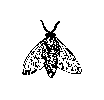
\epsfig{file=fly.eps}
\caption{A sample black and white graphic (.eps format).}
\end{figure}

\begin{figure}
\centering
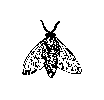
\epsfig{file=fly.eps, height=1in, width=1in}
\caption{A sample black and white graphic (.eps format)
that has been resized with the \texttt{epsfig} command.}
\end{figure}


As was the case with tables, you may want a figure
that spans two columns.  To do this, and still to
ensure proper ``floating'' placement of tables, use the environment
\textbf{figure*} to enclose the figure and its caption.
\begin{figure*}
\centering
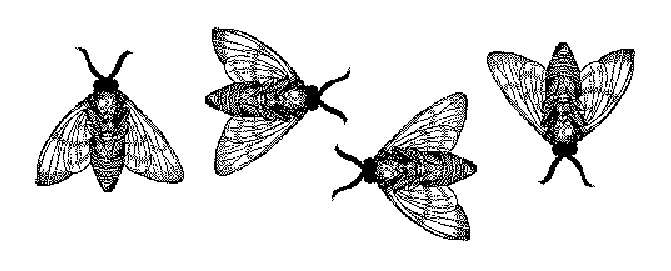
\epsfig{file=flies.eps}
\caption{A sample black and white graphic (.eps format)
that needs to span two columns of text.}
\end{figure*}
and don't forget to end the environment with
{figure*}, not {figure}!

Note that, in this example file, {\textbf{.ps}} or {\textbf{.eps}} formats are
used; use
the \texttt{{\char'134}epsfig} or \texttt{{\char'134}psfig}
commands as appropriate for the different file types. We have also found that
PDF files (as `includable artwork') also works well.

\begin{figure}
\centering
\psfig{file=rosette.ps, height=1in, width=1in,}
\caption{A sample black and white graphic (.ps format) that has
been resized with the \texttt{psfig} command.}
\vskip -6pt
\end{figure}

\subsection{Theorem-like Constructs}
Other common constructs that may occur in your article are
the forms for logical constructs like theorems, axioms,
corollaries and proofs.  There are
two forms, one produced by the
command \texttt{{\char'134}newtheorem} and the
other by the command \texttt{{\char'134}newdef}; perhaps
the clearest and easiest way to distinguish them is
to compare the two in the output of this sample document:

This uses the \textbf{theorem} environment, created by
the\linebreak\texttt{{\char'134}newtheorem} command:
\newtheorem{theorem}{Theorem}
\begin{theorem}
Let $f$ be continuous on $[a,b]$.  If $G$ is
an antiderivative for $f$ on $[a,b]$, then
\begin{displaymath}\int^b_af(t)dt = G(b) - G(a).\end{displaymath}
\end{theorem}

The other uses the \textbf{definition} environment, created
by the \texttt{{\char'134}newdef} command:
\newdef{definition}{Definition}
\begin{definition}
If $z$ is irrational, then by $e^z$ we mean the
unique number which has
logarithm $z$: \begin{displaymath}{\log e^z = z}\end{displaymath}
\end{definition}

Two lists of constructs that use one of these
forms is given in the
\textit{Author's  Guidelines}.
 
There is one other similar construct environment, which is
already set up
for you; i.e. you must \textit{not} use
a \texttt{{\char'134}newdef} command to
create it: the \textbf{proof} environment.  Here
is a example of its use:
\begin{proof}
Suppose on the contrary there exists a real number $L$ such that
\begin{displaymath}
\lim_{x\rightarrow\infty} \frac{f(x)}{g(x)} = L.
\end{displaymath}
Then
\begin{align*}
l=\lim_{x\rightarrow c} f(x) &= \lim_{x\rightarrow c}{\left[ g{x} \cdot {\frac{f(x)}{g(x)}} \right]}\\
&= \lim_{x\rightarrow c} g(x) \cdot \lim_{x\rightarrow c}{\frac{f(x)}{g(x)}} = 0\cdot L = 0, \\
\end{align*}
which contradicts our assumption that $l\neq 0$.
\end{proof}

Complete rules about using these environments and using the
two different creation commands are in the
\textit{Author's Guide}; please consult it for more
detailed instructions.  If you need to use another construct,
not listed therein, which you want to have the same
formatting as the Theorem
or the Definition\cite{salas:calculus} shown above,
use the \texttt{{\char'134}newtheorem} or the
\texttt{{\char'134}newdef} command,
respectively, to create it.

\subsection*{A {\secit Caveat} for the \TeX\ Expert}
Because you have just been given permission to
use the \texttt{{\char'134}newdef} command to create a
new form, you might think you can
use \TeX's \texttt{{\char'134}def} to create a
new command: \textit{Please refrain from doing this!}
The \textit{research4cacm} class file is quite complex and there is the
risk that you may re\texttt{def}ine something. So, please remember, if you choose
to use \texttt{{\char'134}def}, please be careful as recompilation will
be, to say the least, problematic.

% Additional text inserted here to expand the sample to 8 pages
% ------------------------------------------------------------
\section{More text}\label{sec:more-text}

We also illustrate the effect of Laplacian smoothing on our medial
axis approximation. For Laplacian smoothing we assume that we know the
connectivity ordering of the sample points along the boundary curve
$\partial O$. Every sample point has a predecessor and successor in
this ordering. In Laplacian smoothing every sample point is displaced
halfway toward the average of its predecessor and successor. This
process is repeated iteratively.

Typically, the input points sample a curve bounding a shape. In
sample-based geometry processing, properties of shapes can be
discovered by processing this point set, i.e., computing the
Voronoi diagram, the Delaunay triangulation, or more complicated
geometric structures. In Mesecina, such structures are offered for
visualization as \emph{layers}. Currently, there are a total of 41
layers available. Layers can be activated and deactivated, and
properties like color, opacity, point size and line width are easily
modifiable through the user interface.

Unfortunately, the balls in $B_I$ are in general highly degenerate,
i.e., many circles bounding such balls can pass through a single
point. This makes the computation of the restricted power diagram of $B_I$,
and thus the computation of the medial axis prone to
numerical errors.

This gives us an alternative, and numerically more stable way to
compute the medial axis of the union of balls in $B_I$ under the
condition that the smooth boundary $\partial O$ of $O$ is sampled
sufficiently densely.

The goal is to construct energy-efficient schedules, using lower processing speeds, while still
guaranteeing a determined service. (2)~{\em Sleep states\/}: When a system is
idle, it can be put into a low-power sleep state. One has to find out when to
shut down a system, taking into account that a transition back to the active
mode requires extra energy.

{\bf Our contribution:} We present the first algorithm-based study of
multi-processor speed scaling where jobs may have individual release dates and
deadlines. Most of our paper concentrates on the offline scenario. In the first
part of the paper we settle the complexity of the problem with unit size jobs.
We may assume w.l.o.g.\ that $p(i)=1$, for all $i$.  We prove that if job
deadlines are {\em agreeable\/}, an optimal multi-processor schedule can be
computed in polynomial time. In practice, instances with agreeable deadlines
form a natural input class where, intuitively, jobs arriving at later times may
be finished later. Formally, deadlines are agreeable if, for any two jobs $i$
and $i'$, relation $r(i)<r(i')$ implies $d(i)\leq d(i')$. We then show that if
the jobs' release dates and deadlines may take arbitrary values, the energy
minimization problem is NP-hard, even on two processors. For a variable number
of processors, energy minimization is strongly NP-hard. Furthermore, for
arbitrary release dates and deadlines we develop a polynomial time algorithm
that achieves a constant factor approximation guarantee of
$\alpha^\alpha2^{4\alpha}$.

\begin{table*}[t]
\caption{Inventory System Information}
\centering
\begin{tabular}{|r|c|c|c|c|c|c|c|c|c|}  \hline
 & No of & Lines & Mean & Dev Unit & PUT & Total & Fault & Files With & Pct With \\
 Rel & Files & of Code & LOC & Faults & Faults & Faults & Density & Any Faults & Any Faults \\ \hline
 1  &  584 & 145,967 & 250 & 768 & 220 & 988 & 6.78 & 233 & 39.9 \\ \hline
 2  &  567 & 154,381 & 272 & 172 & 28 & 200 & 1.30 & 88 & 15.5 \\ \hline
 3  &  706 & 190,596 & 270 & 400 & 85 & 485 & 2.56 & 140 & 19.8 \\ \hline
 4  &  743 & 203,233 & 274 & 292 & 35 & 327 & 1.61 & 114 & 15.3   \\ \hline
 5  &  804 & 231,968 & 289 & 281 & 56 & 337 & 1.47 & 131 & 16.3  \\ \hline
 6  &  867 & 253,870 & 293 & 288 & 51 & 339 & 1.34 & 115 & 13.3  \\ \hline
 7  &  993 & 291,719 & 294 & 170 & 37 & 207 & 0.71 & 106 & 10.7  \\ \hline
 8  & 1197 & 338,774 & 283 & 375 & 113 & 488 & 1.45 & 148 & 12.4 \\ \hline
 9  & 1321 & 377,198 & 286 & 346 & 88 & 434 & 1.16 & 151 & 11.4  \\ \hline
 10 & 1372 & 396,209 & 289 & 202 & 43 & 245 & 0.62 & 112 & 8.2  \\ \hline
 11 & 1607 & 426,878 & 266 & 174 & 106 & 280 & 0.66 & 114 & 7.1  \\ \hline
 12 & 1740 & 476,215 & 274 & 192 & 81 & 273 & 0.57 & 120 & 6.9  \\ \hline
 13 & 1772 & 460,437 & 260 & 88 & 39 & 127 & 0.28 & 71 & 4.0 \\ \hline
 14 & 1877 & 482,435 & 257 & 164 & 71 & 235 & 0.49 & 95 & 5.1  \\ \hline
 15 & 1728 & 479,818 & 278 & 251 & 54 & 305 & 0.64 & 120 & 6.9  \\ \hline
 16 & 1847 & 510,561 & 276 & 181 & 93 & 274 & 0.54 & 116 & 6.3  \\ \hline
 17 & 1950 & 538,487 & 276 & 188 & 65 & 253 & 0.47 & 122 & 6.3  \\ \hline
\end{tabular}
\label{rel-dens}
\end{table*}

Denote the bidding function as $b(v)$. We conjecture that the bidding
function is monotonically increasing (we can verify that this is true), so
that the reverse bidding function exists and is increasing, denoted as $%
\eta \left( b\right) $. If one's rivals bid according to such a bidding
function, we can write out its probability of winning $j$th share as%
\[
P_{j}\left( b\right) =\left( _{n-j}^{n-1}\right) F\left( \eta \left(
b\right) \right) ^{n-j}\left[ 1-F\left( \eta \left( b\right) \right) \right]
^{j-1}
\]%
In equilibrium, the winning probability for a bidder with valuation $v$ is%
\[
P_{j}\left( v\right) =\left( _{n-j}^{n-1}\right) F\left( v\right) ^{n-j}
\left[ 1-F\left( v\right) \right] ^{j-1}
\]

Denote $v_{0}\in \left[ \underline{v},\bar{v}\right] $ as a reserve price
(minimal bid) set by the auctioneer. Clearly, an advertiser
with $v<v_{0}$ will not bid.

Denote
\[
\int_{v_{0}}^{\overline{v}}P_{j}\left( v\right) \left[ v-\frac{1-F(v)}{f(v)}%
\right] f(v)dv\equiv \alpha _{j}
\]%
and let $\alpha _{m+1}=0$ for notation convenience. $\alpha _{j}$\ can be
interpreted as the marginal return of $j$th share. The coefficients ($\alpha
_{j} $) are generally determined by the distribution function, the
reservation price, and the number of bidders.

From the above Proposition 1, we can see that the expected profit of the
auctioneer is a linear function of share sizes. Intuitively, one would want
to allocate as much resource as possible to the share with the highest
marginal return. Thus the optimal share structure is ultimately determined by
the rank order of these marginal returns. In below, we show the conditions under
which the marginal return of the largest share is the highest such that
providing just one grand share is optimal.

\section{Some Additional Text}

Table~\ref{rel-dens} provides information on the inventory system.
We observed that, after the first release, less than 20\% of the files contained any faults
at all, discovered at any stage of development.
Therefore, we reasoned, if we could identify these files, substantial
effort could be saved if testers could target these files for particular scrutiny.

All three systems used an integrated version control/change management
system that required a {\em modification request} or MR to be written
any time a change was to be made to the system.
An MR, which is most commonly written by a developer or tester, may
identify either (1) a problem or issue found during internal project testing or
reported by a customer or (2) a required or requested change, such
as a system enhancement or maintenance update.

MRs contain a great deal of information, including a written description
of the reason for the proposed change and a severity rating of 1 through
4 characterizing the importance of the proposed change.
If the request results in an actual change, the MR records the file(s)
that are changed or added to the system and the specific lines of code
that are added, deleted, or modified.
It also includes such information as the date of the change and the
development stage at which the change was made.

Most projects begin MR data collection at the time that the system test phase begins for the
first release, and this was the case for the provisioning system used in our case studies.
The inventory system began data collection far earlier, at the requirements stage, and almost
three quarters of the reported faults were identified during unit testing.
Unlike system testing, which is typically done by professional testers whose sole job function
is to develop and run test cases once the system has been fully integrated, unit testing
is generally performed by developers while they are creating individual files.
In addition, the system test process tends to be far more carefully controlled than the unit
testing phase.

One of the reasons why the testing process has gained such a
denotative importance is the fact that it consumes even
50\% of the expended effort on software development
\cite{Pressman2002}. Thus, the software testing activity is
a critical element on the search of quality assurance of a
software product, aiming to make it more reliable.

\textbf{Learning.} Between periods 0 and 1 seller $M$ receives information
form his buyers. We aggregate the information as follows: Let $\mu _{i}$
denote the measure of buyers who buy product $i\in \left\{ l,h\right\} $
from seller $M$ in period 0. Seller $M$ receives a random signal $%
y_{i}\left( x_{i}\right) \in \left\{ -1,0,1\right\} $ on the type of each
product $i\in \left\{ l,h\right\} $ between periods 0 and 1, where
\begin{eqnarray*}
\Pr \left( y_{i}\left( x_{i}\right) =0\mid x_{i}\right) &=&1-\mu _{i}, \\
\Pr \left( y_{i}\left( x_{i}\right) \in \left\{ -1,1\right\} \mid
x_{i}\right) &=&\mu _{i}.
\end{eqnarray*}%
We can interpret a signal of $0$ as containing no information, or simply the
failure to receive an informative signal. Given that the seller receives a
relevant signal, the probability of the signal being correct is:
\[
\Pr \left( y_{i}\left( x_{i}\right) =x_{i}\mid y_{i}\left( x_{i}\right) \in
\left\{ -1,1\right\} ,x_{i}\right) =\frac{1}{2}+\gamma ,
\]%
where $\gamma \in \left[ 0,\frac{1}{2}\right] $. We can interpret $\gamma $\
as the informativeness of the signal. The event tree in Figure 2 summarizes
the signal structure where $x_{i}^{\prime }\neq x_{i}$.

Given the probabilistic structure, we view this type of system as a
mechanism that computes the posterior beliefs for each product $i$ based on
the signal $y_{i}$ and reports them only to the buyers who have bought from
him in period 0. The posterior for product $i$ given signal $y_{i}$ will be
denoted by
\[
\alpha _{i}\left( y_{i}\right) \equiv \Pr \left( x_{i}=1\mid y_{i}\right) .
\]

A performance analysis of distributing QoS parameters over multiple
entities able to communicate together has been performed in this paper.
In this study, we compared the amount of data exchanged in two scenarios
differentiated on the basis of the negotiation approach in use. Our
analysis points out that the HD architecture seems to be an alternative
operator-centric solution to improve QoS management on network side. In
fact, data exchanged on network side in HD architecture scenario is less
than in UMTS scenario. However, this solution increases the amount of
data exchanged on end terminal side. This amount can be reduced by
adopting network assisted or controlled QoS management approaches.
Noticed that this optimization can also be applied during handover
management. We are currently assessing the performance of our
optimization in such a case.

\begin{eqnarray}
    &&B_{UMTS\_R5}^{Terminal} = 4*S_{QoSd} + 184 \\
    &&B_{UMTS\_R5}^{GGSN} = 12*S_{QoSd} + 552\\
    &&B_{UMTS\_R5}^{SGSN} = 2*(l + 2)*(S_{QoSd} + 46)\\
    &&B_{UMTS\_R5}^{RNC} = 2*S_{QoSd} + 92 \\
    &&B_{UMTS\_R5}^{Network} = (11 + 2*l)*S_{QoSd} + 874 \\ \nonumber
    %\end{eqnarray}
    %\begin{eqnarray}
    %&&B_{DAIDALOS}^{Terminal} = 3*S_{QoSd} + 138 \\
    %&&B_{ DAIDALOS }^{ANQoSB} = 2*(l + 3)*(S_{QoSd} + 46\\
    %&&B_{ DAIDALOS }^{MMSP} =12*S_{QoSd} +552\\
    %&&B_{ DAIDALOS }^{AR} = 2*l*(S_{QoSd} + 46) \\
    %&&B_{ DAIDALOS }^{Network} = 2*(l + 6)*(S_{QoSd} + 46) \\ \nonumber\\
    &&B_{HD}^{Terminal} = 3*S_{QoSd} + l*S_{RM} + (l + 3)*46\\
    &&B_{HD}^{OM} = 3*S_{QoSd} + S_{OM} + 184\\
    &&B_{HD}^{IPAM} = 3*S_{QoSd} + S_{OM} + l*(S_{RM}{} \nonumber \\
    & & {} + S_{IPAM}) + (l + 4)*46  \\
    &&B_{HD}^{RM} = 4*S_{QoSd} + 2*S_{RM} + S_{IPAM} + 276\\
    &&B_{HD}^{Network} = 8*S_{QoSd} + S_{OM} + l*S_{IPAM} {} \nonumber \\
    & & {}+ 2*S_{RM} + (2*l + 9)*46
\end{eqnarray}%}

We begin by describing the notation used
in this paper.
The network is represented as the AS graph
$G = (V, E)$, where each node $v \in V$
corresponds to one AS, and each edge $\{u,v\} \in E$
corresponds to a \emph{BGP session} between ASes
$u$ and $v$, meaning that these ASes are physically connected
and share route advertisements.
We assume that links between ASes are reliable FIFO message queues with
arbitrary delays; this accounts for network asynchrony. At most one link
is assumed to exist between ASes, and all the internal and border
routers of an AS are condensed into one node (or one point of
routing-policy control). A path $P$ is a sequence of nodes $v_1 v_2
\cdots v_k$ such that $\{v_i, v_{i+1}\} \in E$; we write $v \in P$ if
path $P$ traverses node $v$. Paths can be concatenated with other nodes
or paths; \emph{e.g.}, if $P = u \cdots v$, $Q = v \cdots w$, and
$\{w,d\} \in E$, we may write $PQd$ to represent the path starting at
node $u$, following $P$ to node $v$, then following $Q$ to node $w$, and
finally traversing the edge $(w, d)$. We assume that paths are directed
from source to destination.
BGP, at a schematic level, computes routes using the following iterative
process: (1) Nodes receive \emph{route advertisements} from their
neighbors, indicating which destinations are reachable and by what
routes; (2) for each destination, a node chooses the best route from
those available, based on local policy; (3) if the current route to a
given destination has changed, an advertisement is sent to neighboring
nodes.

We say the network has converged when each AS $v \in V$ is assigned a
path $\pi(v)$ to the destination, such that the assignment is
\emph{stable}, \emph{consistent} and {\em safe}. By consistent, we mean
that the paths form a forwarding tree to the destination; if $\pi(v) =
vuP$, then $\pi(u) = uP$. By stable, we mean that $\pi(v)$ is the
``best'' available route for each node $v$, given the other nodes' path
assignments, where ``best'' is determined by node $v$'s routing policy;
that is, if $\pi(v)=v\pi(u)$, there is no other node $w$ such that the
path $v\pi(w)$ is more preferred at $v$ than $\pi(v)$.

In this simple example, we note that the router counter does not get propagated beyond the
immediate neighboring pivot. In the detection phase, node {\em B} advertises ({\em BD}:1),
which does not need to be readvertised in the next iteration since {\em B}  receives ({\em CD}:1) thereafter.
As the counter is propagated together with route advertisements, this implies that no
further updates to it will take place in the stable phase.

Considering differences and similarities between both of them,
many open questions are discussed about AO testing, the importance
of the development of a testing model for Aspect--Oriented Programs
(AOPs), and also the inclusion of a potential fault on the model
proposed by Alexander \cite{Alexander2004}.

On an algorithmic level there are two mechanisms to save energy.  (1)~{\em Speed
scaling\/}: Microprocessors currently sold by chip makers such as AMD and Intel
are able to operate at variable speed. The higher the speed, the higher the
power consumption is. Speed scaling techniques dynamically adjust the speed of a
processor executing a set of computing tasks. The goal is to construct
energy-efficient schedules, using lower processing speeds, while still
guaranteeing a determined service. (2)~{\em Sleep states\/}: When a system is
idle, it can be put into a low-power sleep state. One has to find out when to
shut down a system, taking into account that a transition back to the active
mode requires extra energy.

\subsection{A subsection with more text}

Some OO software testing facilities regarding procedural are
presented by McGregor \cite{McGregor1996}: i) methods and classes
interfaces are explicitly defined; ii) lesser number of testing
cases to coverage are resultant, due to the reduced number of
parameters; and iii) reuse of testing cases due to the presence of
the inheritance characteristic. Alexander \cite{Alexander2004} presents specific issues to testing
process over AO paradigm: How to adequately test aspect-oriented
process?

McGregor \cite{McGregor1996} also points out some disadvantages
which must be considered, like: i) the class correctness
evaluation, complicated by the presence of information
encapsulation; ii) the testing management, obstructed by the
multiple entry points (methods) in one class; and iii) object
iterations, expanded by polymorphism and dynamic binding.

Zhao \cite{Zhao2003} proposes a unit testing approach based on
data flow to test AO programs. This approach tests two kinds of
units for AO programs: aspects as modular units that implement
crosscutting concerns, and classes whose behavior could be
affected by one or more aspects. To every unit, three levels of
distinct tests are applied: intra-module, inter-module, and
intra-aspects or intra-classes. Def-use pairs are computed using
Control Flow Graphs (CFG) to define what interactions between
aspects and classes must be tested.

\textit{Case 2:} In this case we assume $a(i+k) < a(i+1)$ and $b(i+k)\leq
b(i+1)$. Our goal is to swap jobs $i+1$ and $i+k$.
To this end we exchange start and finishing times of jobs $i+1$ and $i+k$ as
follows. Let $a'(i+k) := a(i+1)$, $b'(i+k) := b(i+1)$ and $a'(i+1):=a(i+k)$,
$b'(i+1):=b(i+k)$. We can now execute job $i+1$ on processor $(i+1) \bmod m$
(where $i+k$ was scheduled earlier) and job $i+k$ on processor $j$. The new
schedule is feasible since $r(i+1)\leq r(i+k)$ and $d(i+1) \leq d(i+k)$ by the
agreeable deadline property. The energy consumption did not change because the
total energy consumed by $i+1$ and $i+k$ remains unchanged for they have unit
size.

Like some of the characteristics found
on object oriented languages reduce the probability of some
errors, others favor the appearance of new categories of
the same \cite{Binder1999}. Among the favoring characteristics, it
can be cited the encapsulation, polymorphism and dynamic binding.

\textit{Case 3:} For the last case we assume \hbox{$a(i+k) < a(i+1)$} but
$b(i+k)>b(i+1)$. We can now exchange the start times
of jobs $i+1$ and $i+k$ by setting $a'(i+1):= a(i+k)$ and $a'(i+k):= a(i+1)$.
Since start times are exchanged, we can now swap the complete work assignment on
processor $(i+1) \bmod m$ after (and including) job $i+k$ with the work
assignment on processor $j$ after (and including) job $i+1$. The schedule is
feasible since (by agreeable deadlines) $r(i+1) \leq r(i+k)$. The power
consumption of jobs $i+1$ and $i+k$ in the original schedule is
$(b(i+1)-a(i+1))^{1-\alpha}+(b(i+k)-a(i+k))^{1-\alpha}$ while we have
$(b(i+1)-a(i+k))^{1-\alpha}+(b(i+k)-a(i+1))^{1-\alpha}$ in the modified
schedule. By the convexity of the power function the latter expression is
smaller because $a(i+k) < a(i+1)$.

When analyzing {\em CRR\/} on ${\cal J'}$, rather than the optimal schedules
constructed in step~2 of the algorithm, we will consider schedules generated
according to the {\em Average Rate (AVR)} algorithm by Yao.
This algorithm sets processor speeds according to job densities. For any
processor $j$ and time $t$, where $1\leq j \leq m$ and $t\in [0,T)$, let
$c_{kj}(t)$ be the number of jobs from class $C_k$ active at time $t$ that have
been assigned by {\em CRR\/} to processor $j$. Set the speed of processor $j$ at
time $t$ to

\begin{equation}\label{eq:sk}
    s_j(t) = \sum_{k\geq 0} c_{kj}(t)\Delta/2^k.
\end{equation}

Sequencing available jobs on processor $j$ according to the {\em Earliest
Deadline\/} policy yields, not surprisingly, an extremly feasible schedule. Let $S'_{{\mathit AVR},j}$ be the
resulting schedule on processor $j$ and $E'_{AVR,j}$ the energy consumption of
$S'_{\mathit AVR,j}$. As {\em CRR\/} computes an optimal schedule for each
processor, its total energy $E'_{CRR}$ is bounded by
$$
    E'_{CRR} \leq \sum_{j=1}^m E'_{AVR,j}.
$$
We next estimate the energy volumes $E'_{AVR,j}$,
$1\leq j \leq m$. To this end we consider two energy bounds. Firstly, suppose
that job $i'\in {\cal J'}$ is processed at speed $1/(d(i')-r(i'))$ throughout
its active interval. The minimum energy necessary to complete the job is
$(d(i')-r(i'))^{1-\alpha}$ and hence the minimum energy necessary to complete
all jobs $i'\in {\cal J'}$ is at least
\begin{equation}\label{eq:emin}
    E'_{\min}
    = \sum_{i'\in {\cal J'}} (d(i')-r(i'))^{1-\alpha}
    = \sum_{k\geq 0}\sum_{i'\in C_k} (2^k/\Delta)^{1-\alpha}.
\end{equation}

Secondly, we consider the single processor schedule $S'_{\mathit AVR}$
constructed by {\em AVR\/} for ${\cal J'}$.  More specifically, at time $t$ the
speed is set to

\begin{equation}\label{eq:st}
    s(t) = \sum_{k\geq 0} c_k(t)\Delta/2^k.
\end{equation}

%
\begin{proof}
On processor $j$ we schedule the jobs in $S_j$ in increasing order of job
number. Thus the jobs are scheduled in non-decreasing order of deadlines.  We
first consider any job $i\in S_j$ with $p(i) \leq L(i)/m$ and then any $i\in
S_j$ with $p(i) > L(i)/m$. In both cases we will prove that the job is finished
by its deadline.

Fix any $i\in S_j$ with $p(i) \leq L(i)/m$. We will show that after the initial
speed setting in step~1 of the speed function definition, the job is finished by
$d(i)$. As the speed can only increase in the adjustment step~2, the lemma then
holds for this job $i$. Let $k$ be the largest integer such that
$\lambda_k^j\leq i$. By time $d(\lambda^j_k)$ a total load of

\begin{align}
    \sum_{l=1}^{k}&\left(2-{1\over m}\right) s^j_l (d(\lambda^j_l) -
    d(\lambda^j_{l-1}))\nonumber\\
    &=  \left(2-{1\over m}\right)\sum_{l=1}^{k} {1\over m}
        {L(\lambda_l^j)-L(\lambda_{l-1}^j)\over d(\lambda_l^j)-d(\lambda_{l-1}^j)}
        (d(\lambda^j_l) - d(\lambda^j_{l-1}))\nonumber\\
    &= \left(2-{1\over m}\right) L(\lambda_k^j)/m\label{eq:L1}
\end{align}
is completed on processor $j$. If $i>\lambda_k^j$, then between time
$d(\lambda^j_k)$ and $d(i)$ a load of

\begin{multline}    \label{eq:L2}
    \left(2-{1\over m}\right) s^j_{k+1} (d(\lambda^j_{k+1}) -
    d(\lambda^j_k))\\
    = \left(2-{1\over m}\right){1\over m} {L(\lambda_{k+1}^j)-L(\lambda_k^j)\over
        d(\lambda_{k+1}^j)-d(\lambda_k^j)} (d(i) - d(\lambda^j_k))\\
    \geq \left(2-{1\over m}\right){1\over m} {L(i)-L(\lambda_k^j)\over d(i)-d(\lambda_k^j)}
        (d(i) - d(\lambda^j_k))\\
    = \left(2-{1\over m}\right) (L(i)-L(\lambda_k^j))/m
\end{multline}
is completed. The inequality follows from the definition of $\lambda^j_{k+1}$.
Combining (\ref{eq:L1}) and (\ref{eq:L2}) we find that a total load of at least
$(2-{1\over m})L(i)/m$ is finished on processor $j$ by time $d(i)$. It remains
to argue that the total processing requirement of jobs scheduled on processor
$j$ before job $i$ and including $p(i)$ is at most $(2-{1\over m})L(i)/m$.  To
this end consider the event when {\em EDL\/} assigns job $i$ to processor $j$.
As the job is placed on the least loaded processor, just after the assignment
processor $j$ has a load of at most ${1\over m} \sum_{i'<i}p(i') + p(i) \leq
(2-{1\over m})L(i)/m$, and we are done because jobs assigned to processor $j$ at
a later stage are scheduled after job $i$.

Next we examine a job $i$ with $p(i) > L(i)/m$. After the speed adjustment in
step~2 of the speed function definition, processor $j$ runs at a speed of at
least $(2-{1\over m}) p(i)/d(i)$ throughout $[0,d(i))$. Thus a total work of at
least $(2-{1\over m})p(i)$ gets finished by $d(i)$. Again, when {\em EDL\/}
assigns job $i$ to processor $j$, the total load on the processor is upper
bounded by ${1\over m} \sum_{i'<i}p(i') + p(i) \leq (2-{1\over m})p(i)$ and this
is indeed the total work of jobs scheduled on processor $j$ up to (and
including) job $i$.
\end{proof}

We compare the energy incurred by the speed function to the energy of an optimal
solution.  Let

$$
    E_j^1 = \sum_{l=1}^{l_j} (s^j_l)^{\alpha} (d(\lambda^j_l) - d(\lambda^j_{l-1})).
$$

This expression represents the energy used by our speed function on processor
$j$ after the initial setting when speeds are reduced by a factor of $2-{1\over
m}$.

Given an optimal schedule, let $s_{l,{\rm opt}}$ be the average speed of the $m$
processors during the time interval $[d(\lambda^j_{l-1}), d(\lambda^j_l))$, for
$l=1, \ldots, l_j$. By the convexity of the power function, the total energy
used by the optimal solution is

$$
    E_{{\rm OPT}}
    \geq m \sum_{l=1}^{l_j} (s_{l,{\rm opt}})^{\alpha} (d(\lambda^j_l)- d(\lambda^j_{l-1})).
$$

The speeds $s_{l,{\rm opt}}$ must satisfy the constraint that at time
$d(\lambda^j_k)$ a load of at least $L(\lambda^j_k)$ is completed, for $k=1,
\ldots, l_j$. In the following let $\delta^j_l= d(\lambda^j_l)-
d(\lambda^j_{l-1})$.
%We next show that the speeds $s^j_l$, with $1\leq l \leq
%l_j$, defined in (\ref{eq:speed}) minimize the function $f(x_1,\ldots,x_{l_j}) =
%m \sum_{l=1}^{l_j} x_l^{\alpha} \delta^j_l$ subject to the constraint

\begin{equation}\label{eq:const}
    m \sum_{l=1}^k x_l \delta^j_l \geq L(\lambda^j_k),
\end{equation}
for $k=1, \ldots, l_j$.  Suppose $(y_1, \ldots, y_{l_j})$ with  $(y_1, \ldots,
y_{l_j}) \neq (s^j_1, \ldots, s^j_{l_j})$ is an optimal solution. Note that

\begin{equation}\label{eq:load}
    m \sum_{l=1}^k s^j_l \delta^j_l = L(\lambda^j_k),
\end{equation}
for $k=1, \ldots, l_j$. Thus there must exist a $k$ with $y_k > s_k^j$: If $y_l
\leq s_l^j$ held for $l=1, \ldots, l_j$, then there would be a $k'$ with $y_{k'}
< s_{k'}^j$ and hence $m \sum_{l=1}^{k'} y_l^{\alpha} \delta^j_l <
L(\lambda^j_{k'})$, resulting in a violation of constraint (\ref{eq:const}) for
$k=k'$.  Let $k_1$ be the smallest index such that $y_{k_1} > s_{k_1}^j$. We
have $y_l = s^j_l$, for $l=1, \ldots, k_1-1$ since otherwise, using the same
argument as before, constraint (\ref{eq:const}) would be violated for $k=k_1-1$.
Let $k_2$ with $k_2 > k_1$ be the smallest index such that $y_{k_1}> y_{k_2}$.
Such an index exists because otherwise the invariant implies $y_l
> s^j_l$, for $l=k_1, \ldots, l_j$, and we find $m \sum_{l=1}^{l_j} y_l
\delta^j_l > L(\lambda^j_{l_j})$. In this case we could reduce $y_{l_j}$,
achieving a smaller objective function value $f$ and hence a contradiction to
the optimality of the $y_l$, $1\leq l \leq l_j$.
% ------------------------------------------------------------

\section{Conclusions}
This paragraph will, effectively, end the body of this sample document.
You might still have Acknowledgments or an Appendix in your \textit{original}
conference article, however, do remember
(as stated in the Introduction) \textit{Research Highlights}
are purposefully edited so that they appeal to a broader community.
Whilst, for example, explicit proofs of theorems are appropriate, and welcomed, in an
Appendix section for a \textit{Proceedings}, they are inappropriate in the context
of a \textit{magazine}.

There is still the Bibliography to deal with; and
we will make a disclaimer about that here: with the exception
of the reference to the \LaTeX\ book, the citations in
this paper are to articles which have nothing to
do with the present subject and are used as
examples only.

Most authors will avail of a \textit{bibliography database} (\texttt{.bib})
and \texttt{{\char'134}cite} the key values therein. The most appropriate
\textit{bibliography style file} (\texttt{.bst}) to use is the \texttt{abbrv} style.
ACM endorses the use of a \texttt{.bib} and the \texttt{abbrv} style in order
to produce the references. However, because the number of references for a
\textit{Researchh Highlights} article is reduced, we have no
problem with authors choosing, instead, to enter their references \textit{directly} using
a \texttt{{\char'134}bbl}.

%ACKNOWLEDGMENTS are optional
\section{Acknowledgments}
This section is optional; it is a location for you
to acknowledge grants, funding, editing assistance, collaboration, access to
uncommon, but necessary, hardware or software etc.
In the present case, for example, the
authors would like to thank Gerald Murray of ACM for
his help in codifying this \textit{Author's Guide}
and the \textbf{.cls} and \textbf{.tex} files that it describes.


% The following two commands are all you need in the
% initial runs of your .tex file to
% produce the bibliography for the citations in your paper.
\bibliographystyle{abbrv} % standard abbrv style
\bibliography{bibs4cacm}  % substitute the name of 'your' Bibliography here
% You must have a proper ".bib" file
% and remember to run:
% latex bibtex latex latex (in that particular order) in order to resolve all the 'numerical values'
% be they for figures, equation numbers, references, footnotes, etc. etc.
%
\balancecolumns
% That's all folks! % GM Sept. 2008
\end{document}
